\section{Results}
Figure \ref{fig:Results1} shows the number of steps taken per epoch by two agents using single or team agent Q-learning for a run of 3000 epochs. Each plot shows a graph of the number of steps it takes for the agents to reach and grab the block and a graph of the number of steps it takes them to move the block to the goal. We measured the difference in performance between the two Q-learning algorithms by both the speed at which the amount of steps is approximately converged, and the optimality of the learned solution. 

\begin{figure}
	\centering
	\begin{subfigure}{.48\textwidth}
		\centering
		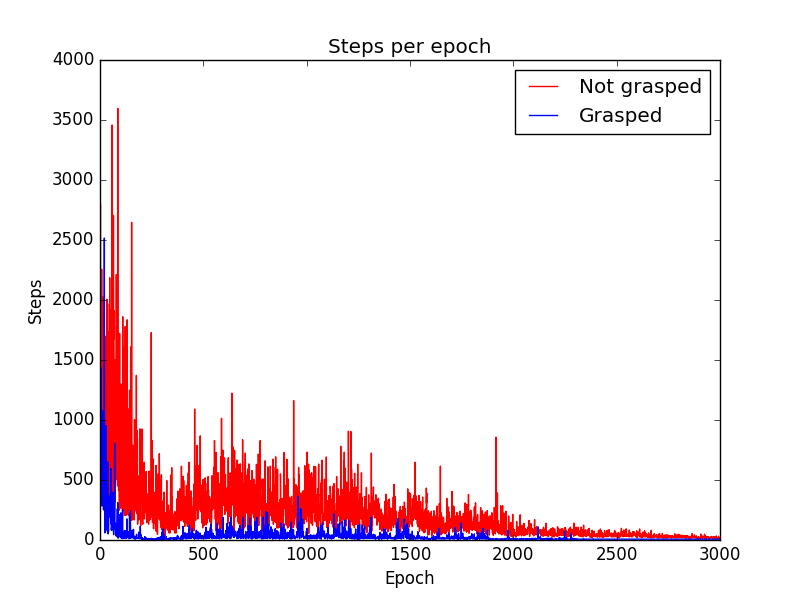
\includegraphics[width=\textwidth]{images/SingleQ.png}
		\caption{Single Q}
	\end{subfigure}
	\begin{subfigure}{0.48\textwidth}
		\centering
		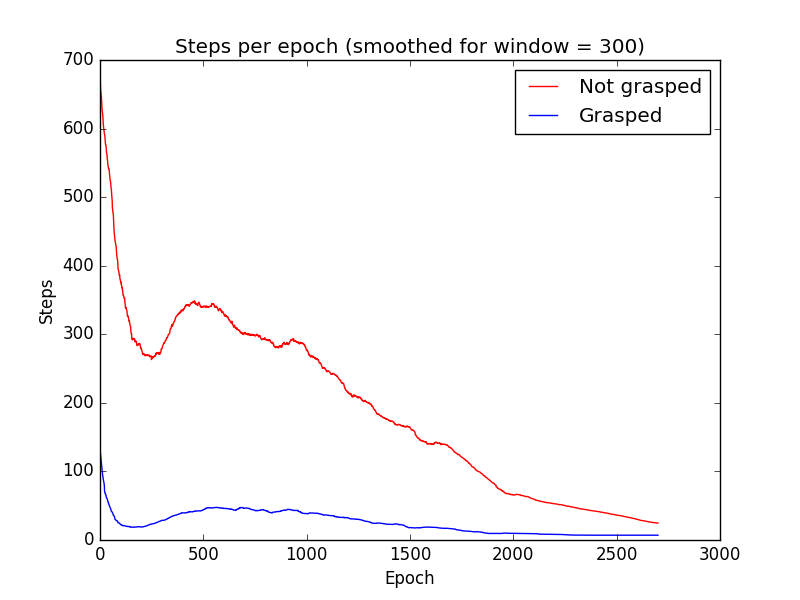
\includegraphics[width=\textwidth]{images/SingleQ_smoothed.png}
		\caption{Single Q (smoothed)}
	\end{subfigure}
	\begin{subfigure}{.48\textwidth}
		\centering
		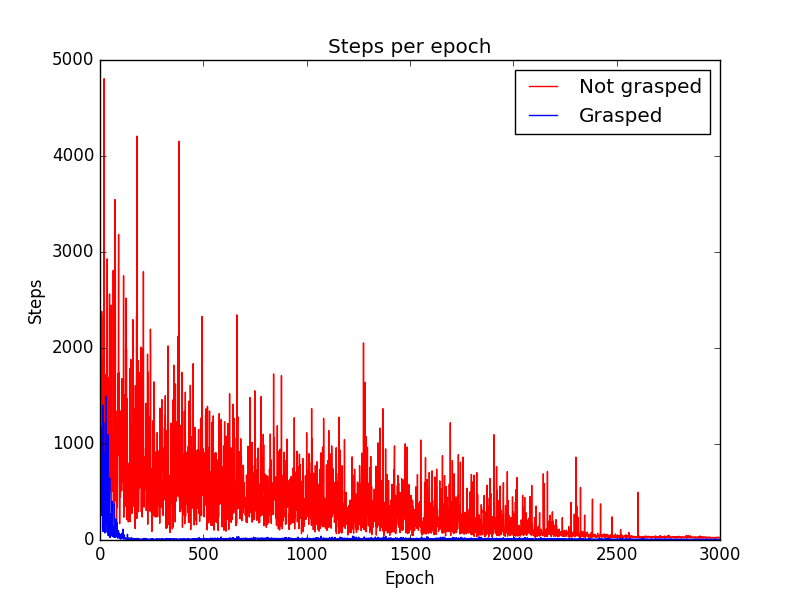
\includegraphics[width=\textwidth]{images/TeamQ.png}
		\caption{Team Q}
	\end{subfigure}
	\begin{subfigure}{0.48\textwidth}
		\centering
		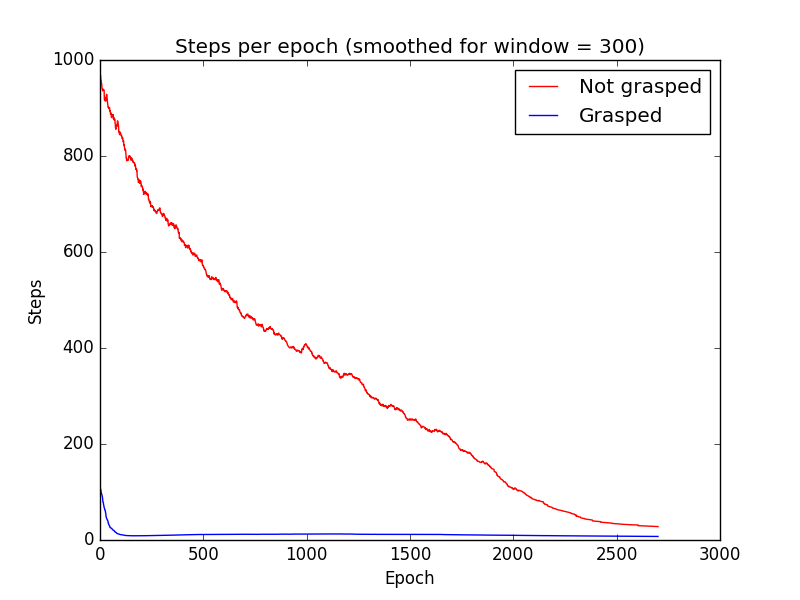
\includegraphics[width=\textwidth]{images/TeamQ_smoothed.png}
		\caption{Team Q (smoothed)}
	\end{subfigure}
	\caption{Number of steps over 3000 epochs}
	\label{fig:Results1}
\end{figure}


\subsection{Speed of convergence}
To measure the speed of convergence we used as a convergence criterion that the standard deviation of 20 consecutive epochs be smaller than a set value.\footnote{For these results $\sigma_{not_grabbed} < 7$ and $\sigma_{grabbed} < 2$.} Figures \ref{3a} and \ref{3b} show the standard deviations for both the single and team learning algorithm. The simulation was run 30 times per learning algorithm and every run the number of epochs it took to reach the convergence criterion was counted. Figures \ref{3c} and \ref{3d} show the results of these counts per condition (grabbed or not grabbed).

To test whether the difference was significant we performed an unpaired t-test on the not grabbed, grabbed and summed results. Given a 95 percent confidence interval the t-test tested significant for the not grabbed samples with $m_{single} \approx 2609$ and $m_{team} \approx 2512$: $t(44.223) = 2.8123$, $p < 0.05$. It tested highly significant for the grabbed samples, with $m_{single} = 1772$ and $m_{team} = 290.4$: $t(52.353) = 14.032$, $p<0.001$. Finally, the t-test tested highly significant for the added results, with $m_{single} \approx 4381$ and $m_{team} \approx 2802$: $t(49.721) = 14.672$, $p < 0.001$. 
\begin{figure}
	\centering
	\begin{subfigure}{.48\textwidth}
		\centering
		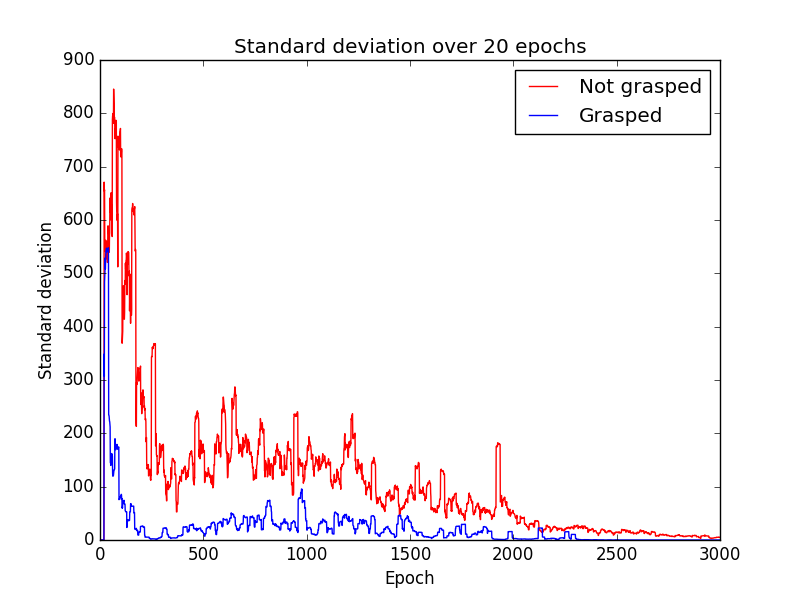
\includegraphics[width=\textwidth]{images/Stdev_single.png}
		\caption{Single Q}
		\label{3a}
	\end{subfigure}
	\begin{subfigure}{0.48\textwidth}
		\centering
		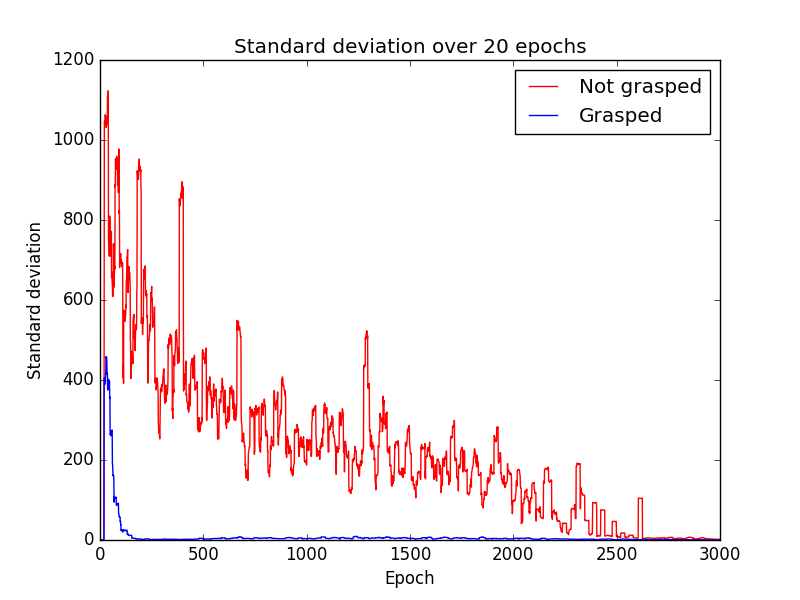
\includegraphics[width=\textwidth]{images/Stdev_team.png}
		\caption{Team Q}
		\label{3b}		
	\end{subfigure}
	\begin{subfigure}{.48\textwidth}
		\centering
		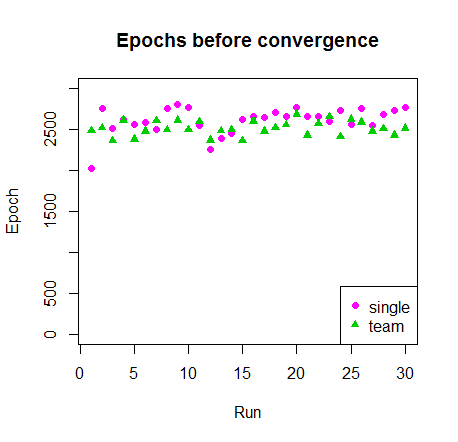
\includegraphics[width=\textwidth]{images/Convergence_notgrabbed.png}
		\caption{Not grabbed}
		\label{3c}		
	\end{subfigure}
	\begin{subfigure}{0.48\textwidth}
		\centering
		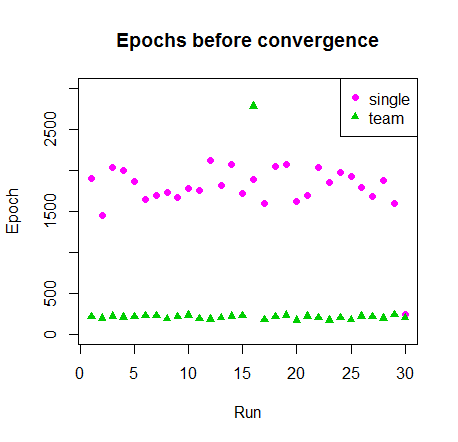
\includegraphics[width=\textwidth]{images/Convergence_grabbed.png}
		\caption{Grabbed}
		\label{3d}		
	\end{subfigure}
	\caption{(a and b) Standard deviation over 20 epochs in a run of 3000 epochs. (c and d) Epochs before convergence.}
	\label{fig:Results3}
\end{figure}

From these results we can conclude that single Q-learning is converged slightly faster when the block is not grabbed, but considerably slower when the block is grabbed. In total this results in the team Q-learning being quite faster overall, with an average difference of approximately 1597 epochs. Note that this difference is taken over the sum of the epochs for grabbed and not grabbed samples. Since the algorithms do both the grabbed and not grabbed part during one epoch, you might also consider just the difference between the samples with the highest number of epochs, which in both cases is the not grabbed one. This difference was still measured highly significant, but is much smaller: ca. 97 epochs.

\subsection{Solution optimality}
To determine how good the found solutions were, we calculated the average number of steps taken in the final twenty epochs that showed a standard deviation under the threshold value, as discussed in the previous section. Figure \ref{fig:Results4} shows the average number of steps taken in the grabbed and non grabbed scenario by both of the Q-learning algorithms.

Again we performed an unpaired t-test on these results. This tested highly significant for the not grabbed samples with $m_{single} \approx 31.9$ and $m_{team} \approx 38.1$: $t(56.961) = -5.2118$, $p < 0.001$. For the grabbed samples the test did not test significantly with $m_{single} \approx 8.66$ and $m_{team} \approx 8.99$: $t(57.428) = -1.9165$, $p > 0.05$. Finally for the total number of steps the test tested highly significant with $m_{single} \approx 40.6$ and $m_{team} \approx 47.1$: $t(56.165) = -5.4113$, $p < 0.001$.

\begin{figure}
	\centering	
	\begin{subfigure}{.48\textwidth}
		\centering
		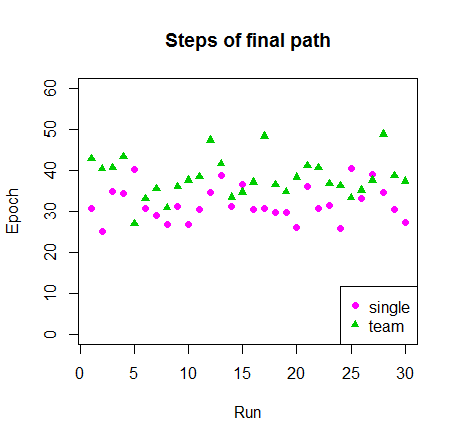
\includegraphics[width=\textwidth]{images/Path_notgrabbed.png}
		\caption{Not grabbed}
		\label{4c}		
	\end{subfigure}
	\begin{subfigure}{0.48\textwidth}
		\centering
		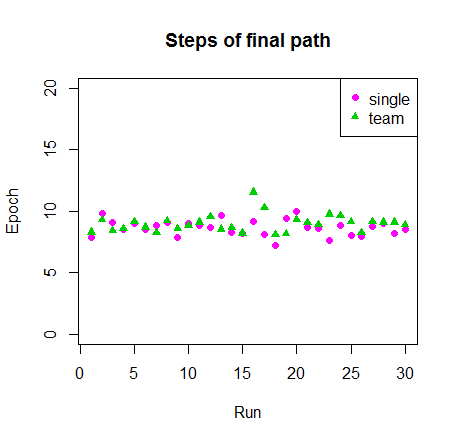
\includegraphics[width=\textwidth]{images/Path_grabbed.png}
		\caption{Grabbed}
		\label{4d}		
	\end{subfigure}
	\caption{Average number of time steps taken for the agents to solve the problem.}
	\label{fig:Results4}
\end{figure}

These results show that, within the number of epochs in which the algorithms converge to below the predefined threshold, on average the single agent Q-learning algorithm finds the better solution for the first stage of the simulation in which the agents have to find the block and grab it. for the second stage, in which the agents have to move the block, there was no significant difference between the two algorithms. Overall however, because of the difference in the first stage, the single agent algorithm performed significantly better: the agents finished the simulation in approximately 6.5 steps less than with the team algorithm.